\pagenumbering{roman}

\subsection{Features Analysis in Depth}
\label{app:features-analysis-in-depth}

\begin{longtable}{P{0.45\textwidth}P{0.45\textwidth}}
\caption{Feature Analysis} 
\label{table:featureAnalysis}
\\ \hline
\textbf{Feature Analysis} & \textbf{Frequency Distribution} \\ \hline 
\textbf{Sex} & \\
Sex is the sex of the patient. It's a binary variable with the following meaning:
\begin{description}
    \item[1] Female;
    \item[2] Male.
\end{description}
The distribution is almost 50-50 (50.07\% females and 49.93\% male). 
& 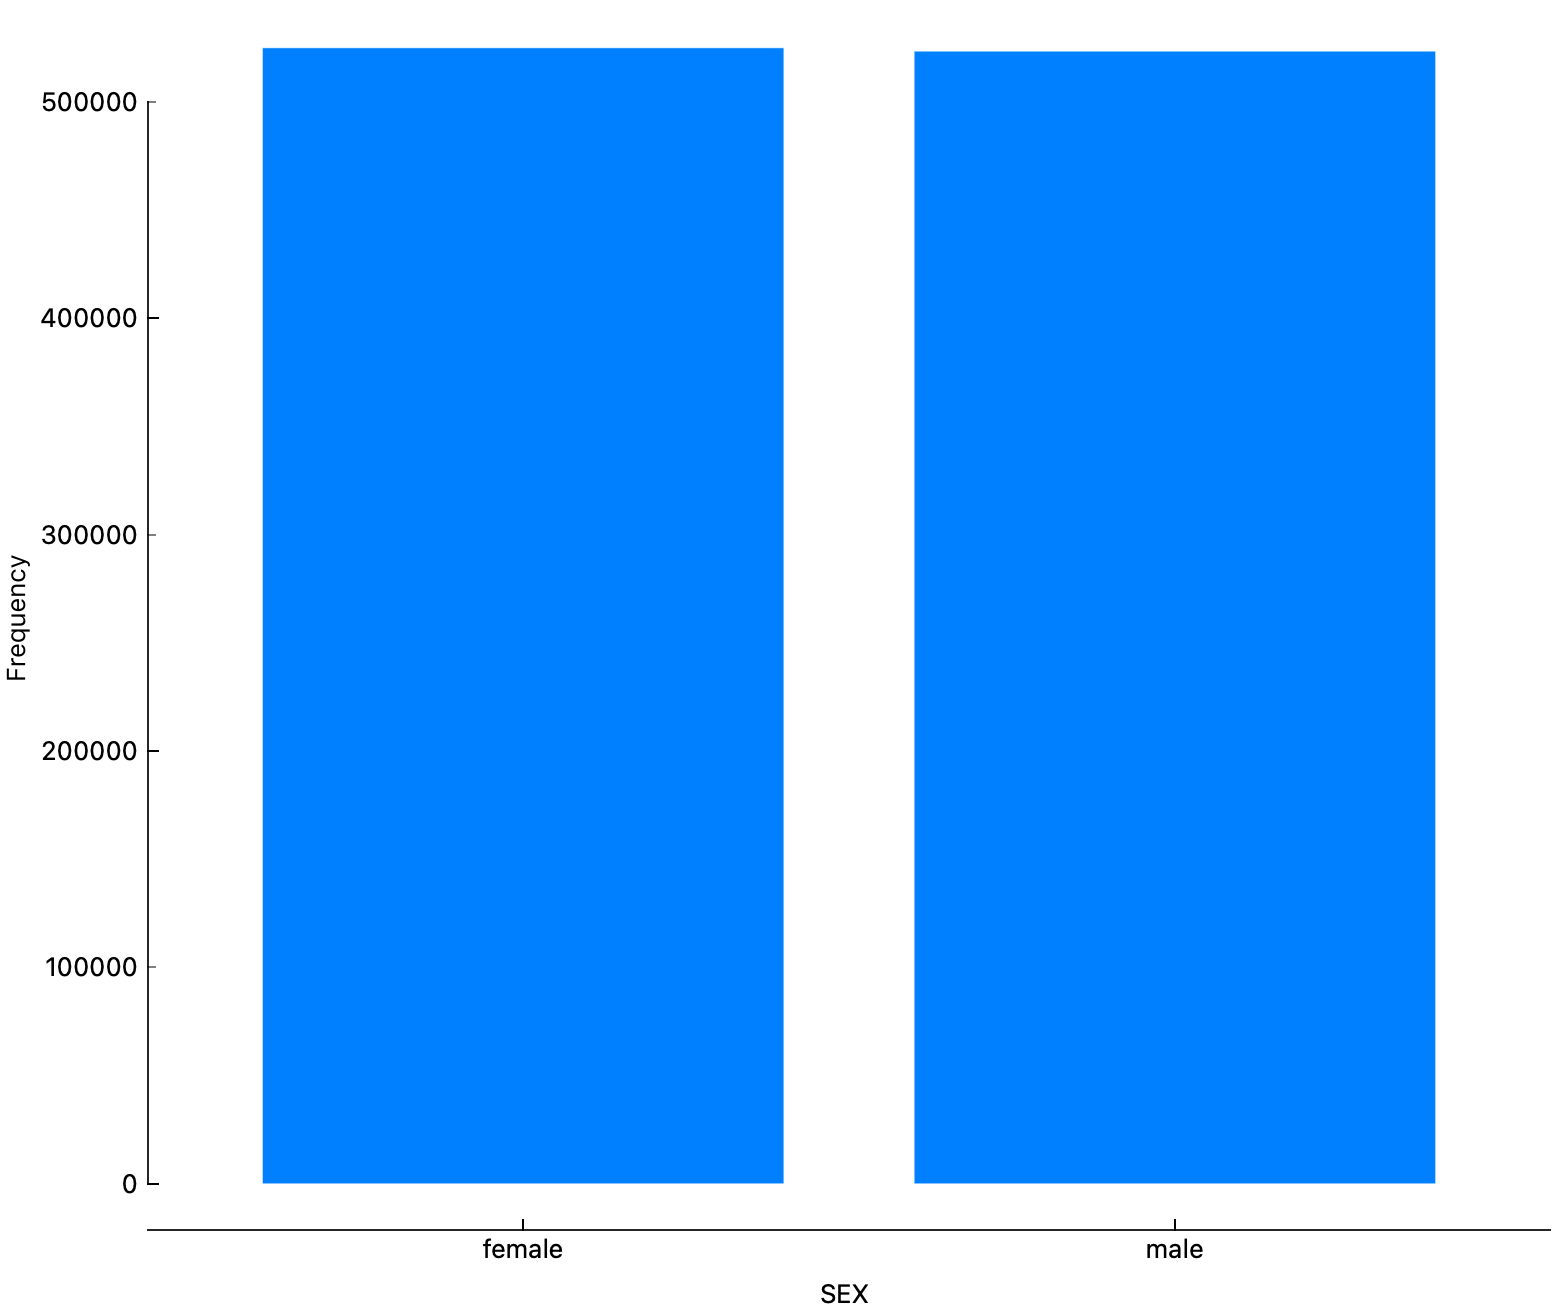
\includegraphics[width=0.44\textwidth]{img/appendix/feature_sex.png} 
\\ \hline
\textbf{Age} & \\
Age is the age of the patient. It's a numeric variable and we can tell that is composed 
by mainly adults. The dataset is fairly distributed by age and sex.
& 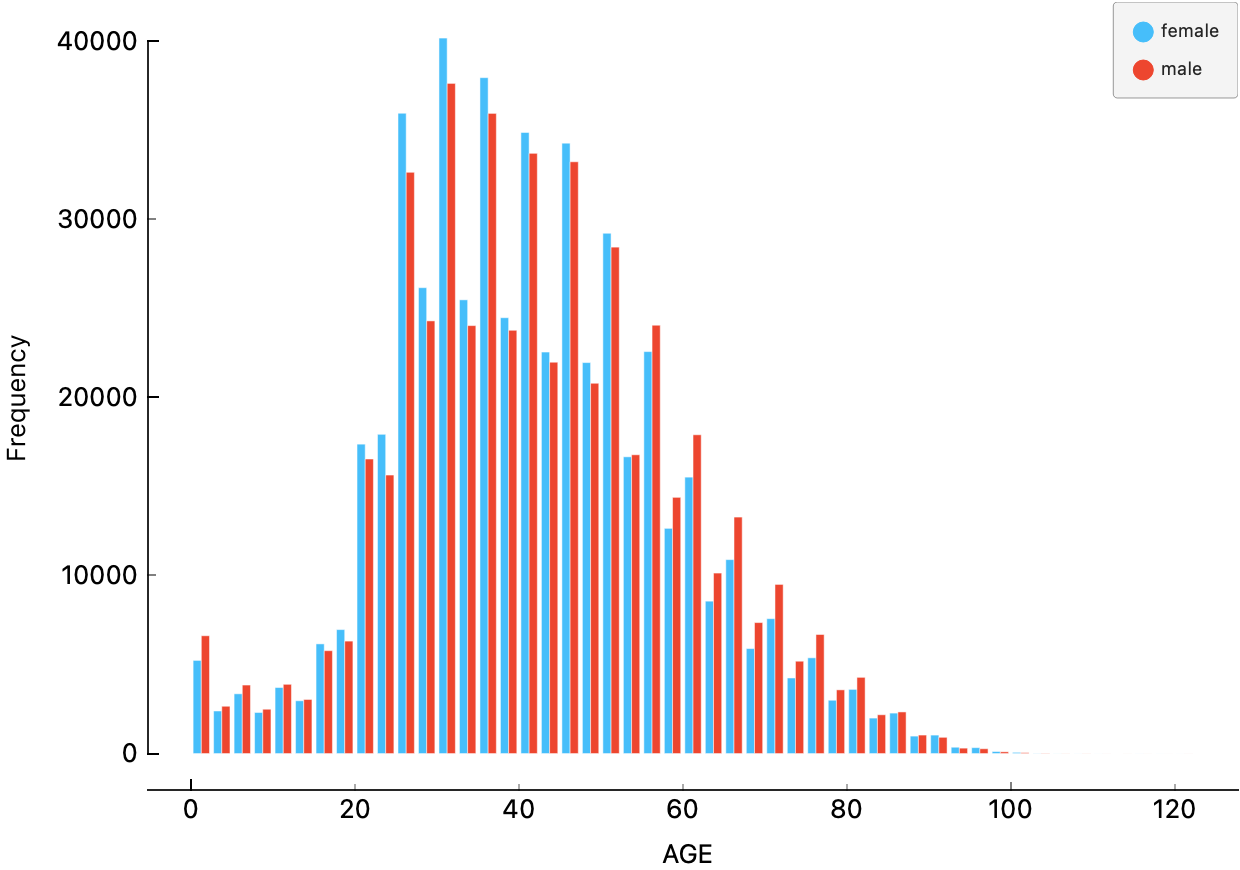
\includegraphics[width=0.44\textwidth]{img/appendix/feature_age_by_sex.png} 
\\ \hline
\textbf{Classification} & \\
Classification is the diagnosis based on the COVID-19 test result. Has a range of values 1-7. Where 1 means that the patient has 1 degree COVID-19 and 7 it has no COVID-19/inconclusive. So we have:
\begin{description}
    \item[1-3] The patient has COVID-19 (degrees 1 to 3);
    \item[4-7] The patient is not a carrier of COVID-19 or the test is inconclusive.
\end{description}
The most predominant values is the level 3 and 7 representing almost 70\% of the data.
& 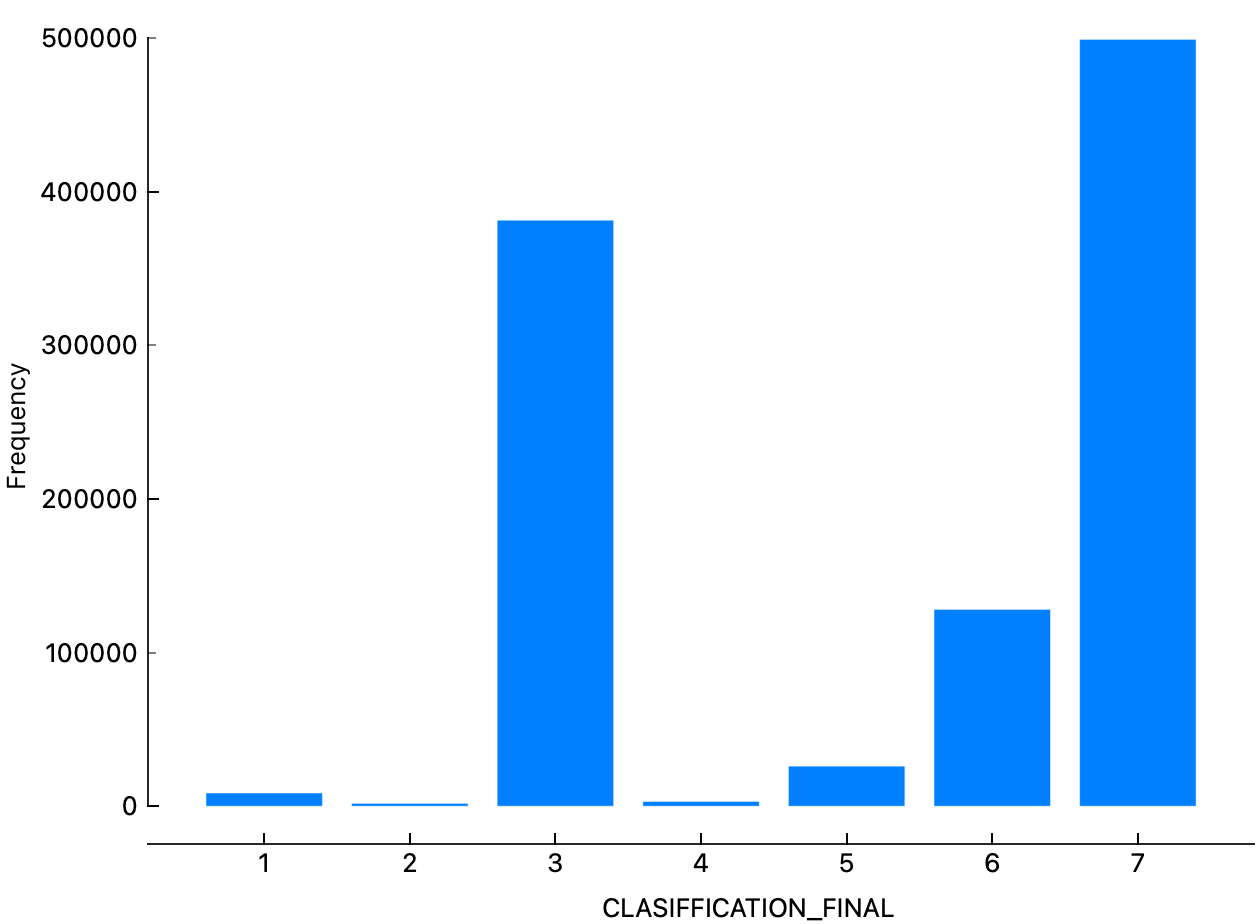
\includegraphics[width=0.44\textwidth]{img/appendix/feature_classification.png} 
\\ \hline
\textbf{Patient Type} & \\
Type of care of the patient received in the unit:
\begin{description}
    \item[1] Returned Home;
    \item[2] Hospitalization.
\end{description}
The most predominant are the patients that returned home.
& 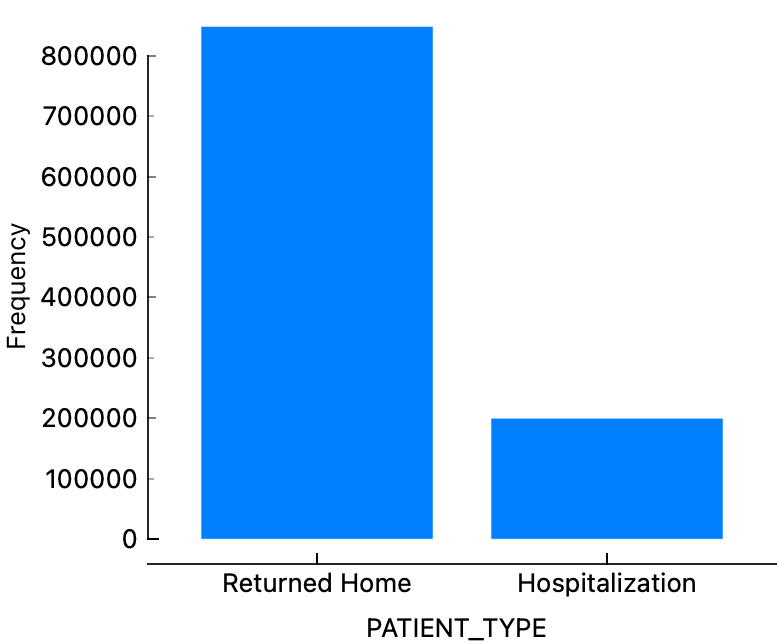
\includegraphics[width=0.44\textwidth]{img/appendix/feature_patient.png} 
\\ \hline
\textbf{Pneumonia} & \\
Pneumonia is a binary variable whether the patient has the inflamation or not.
\begin{description}
    \item[1] Has Pneumonia;
    \item[2] Does not have Pneumonia;
    \item[99] Missing value.
\end{description}
We have around 2\% of missing data and the predominant value is No.
& 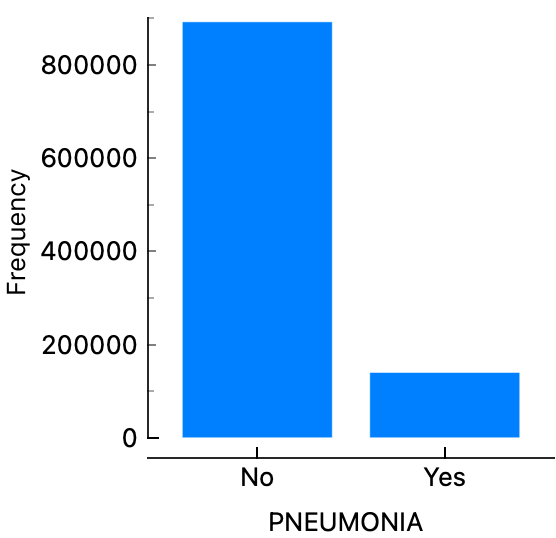
\includegraphics[width=0.44\textwidth]{img/appendix/feature_pneumonia.png} 
\\ \hline
\textbf{Pregnancy} & \\
Pregnancy is a binary variable whether the patient has the inflammation or not.
\begin{description}
    \item[1] Pregnant;
    \item[2] Non Pregnant;
    \item[99] Missing value.
\end{description}
We have around 50\% of missing data (related with the fact
that 50\% are men) and the predominant value is No.
We only have around 1.5\% pregnants.
& 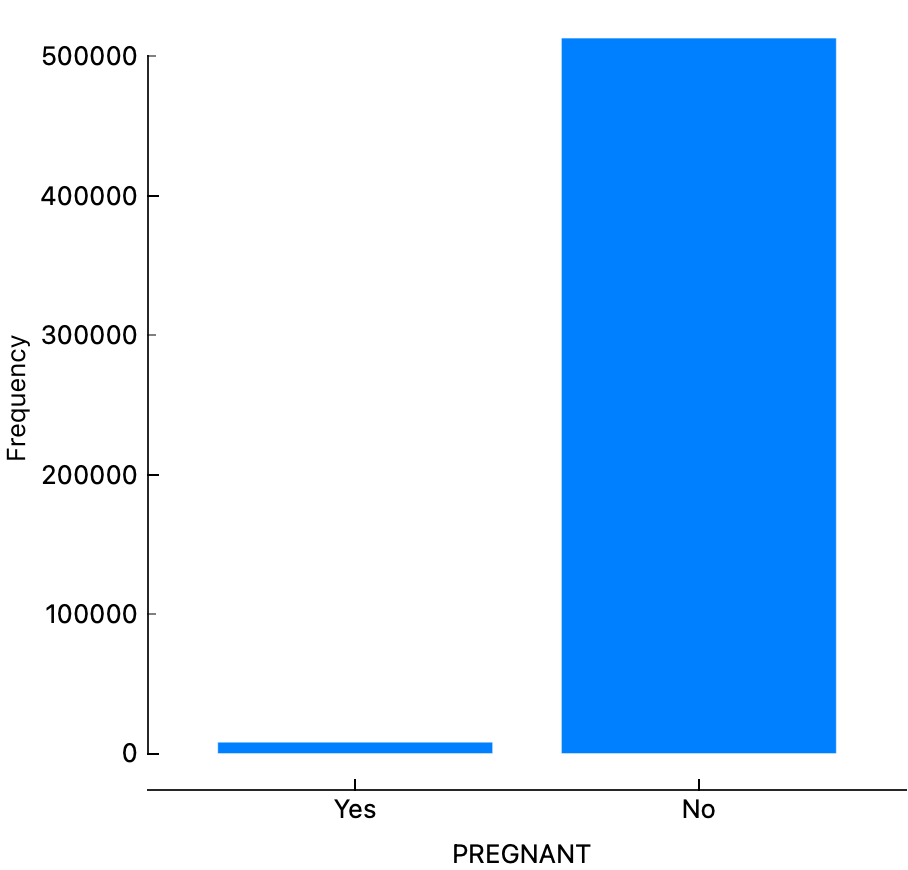
\includegraphics[width=0.44\textwidth]{img/appendix/feature_pregnant.png} 
\\ \hline
\textbf{Diabetes} & \\
Whether the patient has diabetes or not.
\begin{description}
    \item[1] Has Diabetes;
    \item[2] Does not have Diabetes;
    \item[98] Missing value.
\end{description}
We have only 3338 cases with missing data.
And we have 12\% of population with diabetes.
& 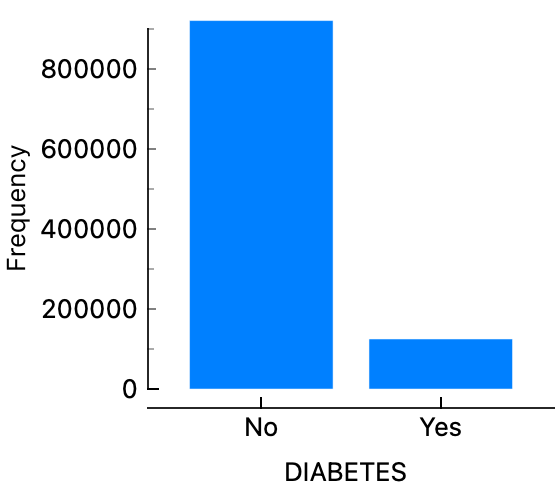
\includegraphics[width=0.44\textwidth]{img/appendix/feature_diabetes.png} 
\\ \hline
\textbf{copd} & \\
copd indicated whether the patient has \emph{Chronic Obstructive Pulmonary 
Disease} or not
\begin{description}
    \item[1] Yes;
    \item[2] No;
    \item[98] Missing value.
\end{description}
We have only 3003 cases with missing data.
And we have 1.44\% of population with copd.
& 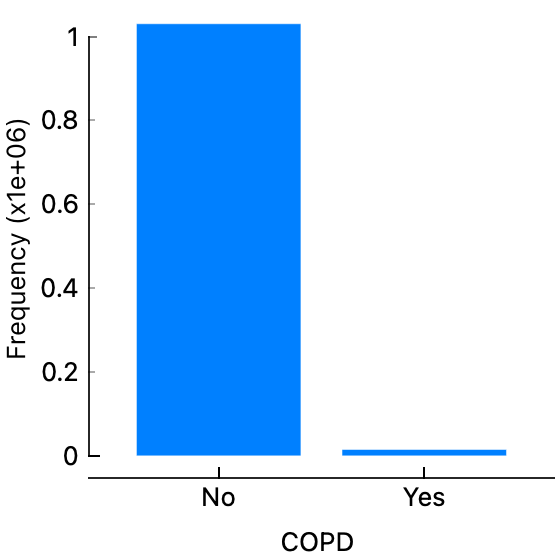
\includegraphics[width=0.44\textwidth]{img/appendix/feature_copd.png} 
\\ \hline
\textbf{asthma} & \\
Whether the patient has asthma or not. Values:
\begin{description}
    \item[1] Yes;
    \item[2] No;
    \item[98] Missing value.
\end{description}
We have 2979 cases with missing data.
And we have 3\% of population with asthma.
& 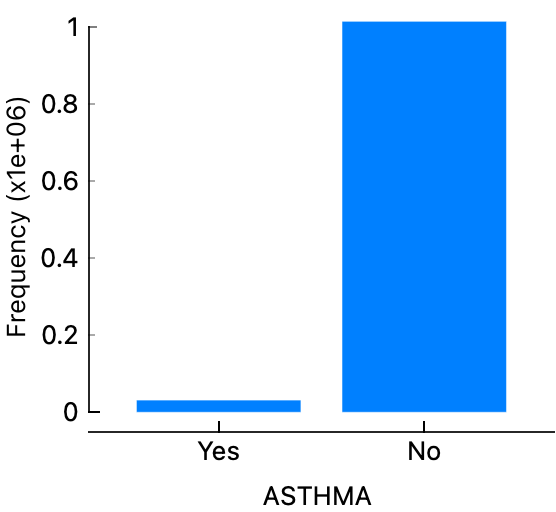
\includegraphics[width=0.44\textwidth]{img/appendix/feature_asthma.png} 
\\ \hline
\textbf{inmsupr} & \\
Whether the patient is immunosuppressed or not. Being immunosuppressed means that a person's immune system is less effective at fighting off diseases and infections. Values:
\begin{description}
    \item[1] Yes;
    \item[2] No;
    \item[98] Missing value.
\end{description}
We have 3404 cases with missing data.
And we have 1\% of population immunosuppressed.
& 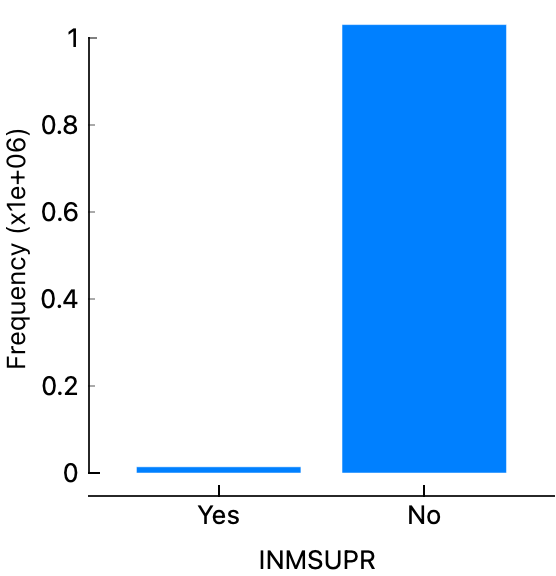
\includegraphics[width=0.44\textwidth]{img/appendix/feature_inmsupr.png} 
\\ \hline
\textbf{Hypertension} & \\
Whether the patient has hypertension or not. Values:
\begin{description}
    \item[1] Yes;
    \item[2] No;
    \item[98] Missing value.
\end{description}
We have 3104 cases with missing data.
And we have 16\% of population with Hypertension.
& 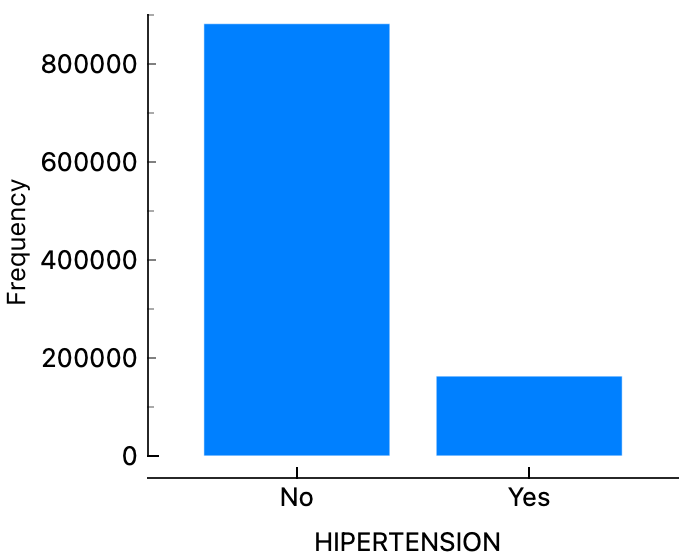
\includegraphics[width=0.44\textwidth]{img/appendix/feature_hypertension.png} 
\\ \hline
\textbf{Cardiovascular} & \\
Whether the patient has heart or blood vessels related disease. Values:
\begin{description}
    \item[1] Yes;
    \item[2] No;
    \item[98] Missing value.
\end{description}
We have 3076 cases with missing data.
And we have 2\% of population has Cardiovascular disease.
& 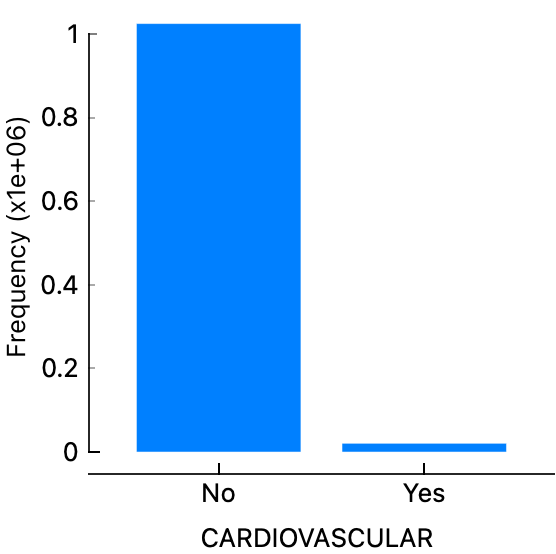
\includegraphics[width=0.44\textwidth]{img/appendix/feature_cardiovascular.png} 
\\ \hline
\textbf{renal chronic} & \\
Whether the patient has chronic renal disease or not. Values:
\begin{description}
    \item[1] Yes;
    \item[2] No;
    \item[98] Missing value.
\end{description}
We have 3006 cases with missing data.
And we have 1.81\% of population has renal disease.
& 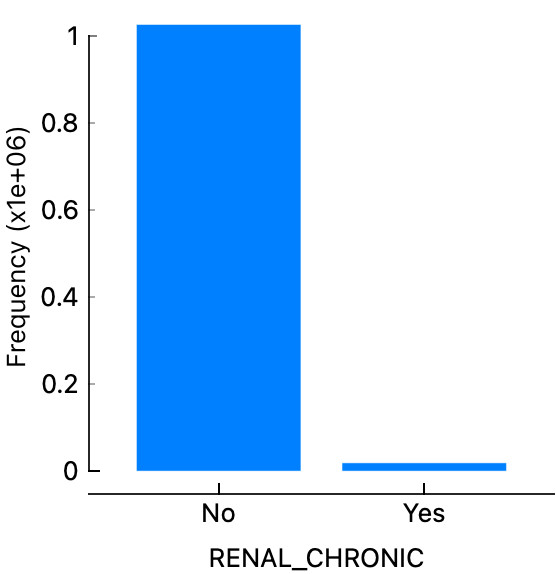
\includegraphics[width=0.44\textwidth]{img/appendix/feature_renal.png} 
\\ \hline
\textbf{other disease} & \\
Whether the patient has other disease or not. Values:
\begin{description}
    \item[1] Yes;
    \item[2] No;
    \item[98] Missing value.
\end{description}
We have 5045 cases with missing data.
And we have 2.7\% of population has other disease.
& 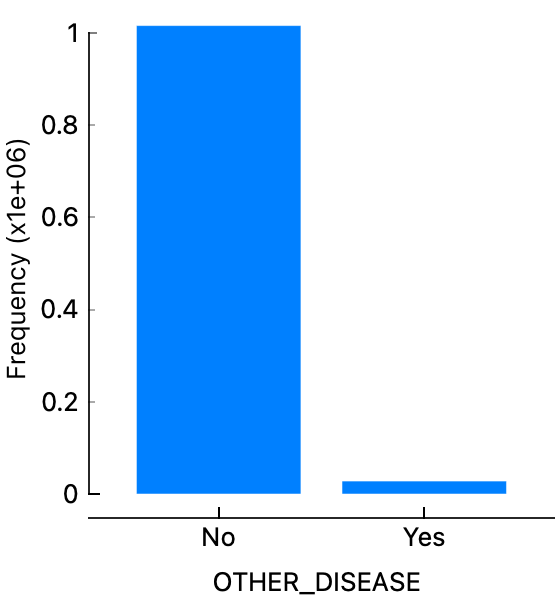
\includegraphics[width=0.44\textwidth]{img/appendix/feature_otherdisease.png} 
\\ \hline
\textbf{Obesity} & \\
Whether the patient is obese or not. Values:
\begin{description}
    \item[1] Yes;
    \item[2] No;
    \item[98] Missing value.
\end{description}
We have 3032 cases with missing data.
And we have 15\% of population is obese.
& 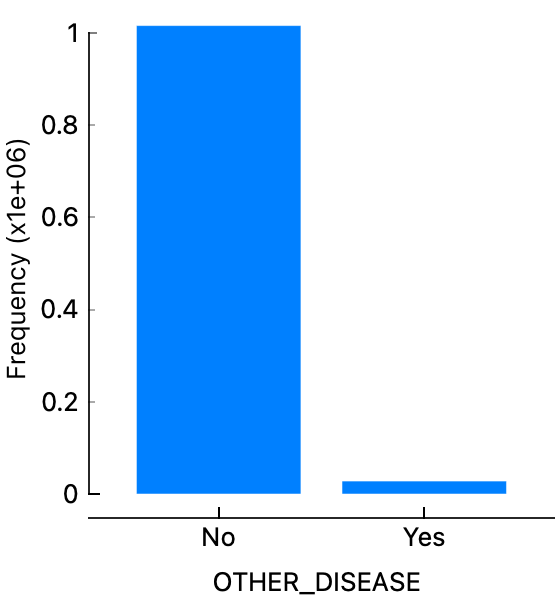
\includegraphics[width=0.44\textwidth]{img/appendix/feature_otherdisease.png} 
\\ \hline
\textbf{tobacco} & \\
Whether the patient is a tobacco user. Values:
\begin{description}
    \item[1] Yes;
    \item[2] No;
    \item[98] Missing value.
\end{description}
We have 3220 cases with missing data.
And we have 8\% of population is obese.
& 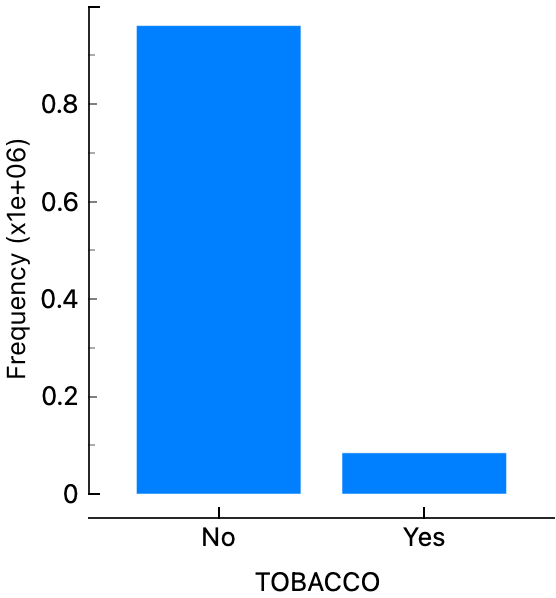
\includegraphics[width=0.44\textwidth]{img/appendix/feature_tobacco.png} 
\\ \hline
\textbf{usmer} & \\
Indicates whether the patient treated medical units of the first, second or third level. Values:
\begin{description}
    \item[1] Yes;
    \item[2] No.
\end{description}
We have no missing data.
And 37\% of population was treated in a medical unit.
& 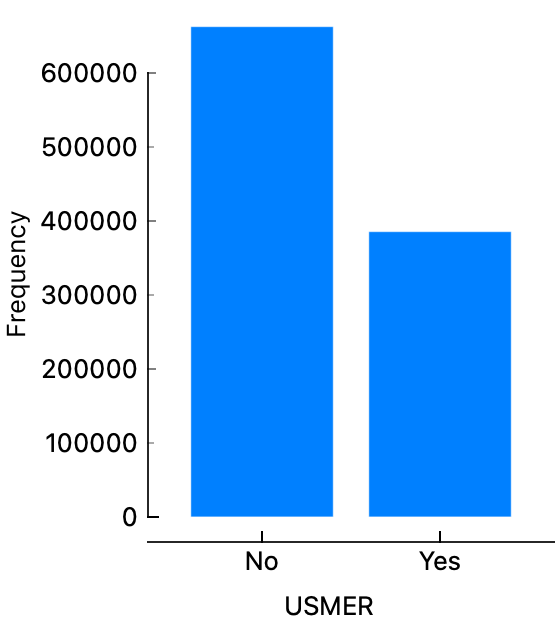
\includegraphics[width=0.44\textwidth]{img/appendix/feature_usmer.png} 
\\ \hline
\textbf{medical unit} & \\
Type of institution of the National Health System that provided the care were
the patients were treated. 
It is a categorical value with 13 Medical Unit Types (Numeric values ranging
between 1 to 13).
We have no missing data.
The predominant data is 12 and 4.
& 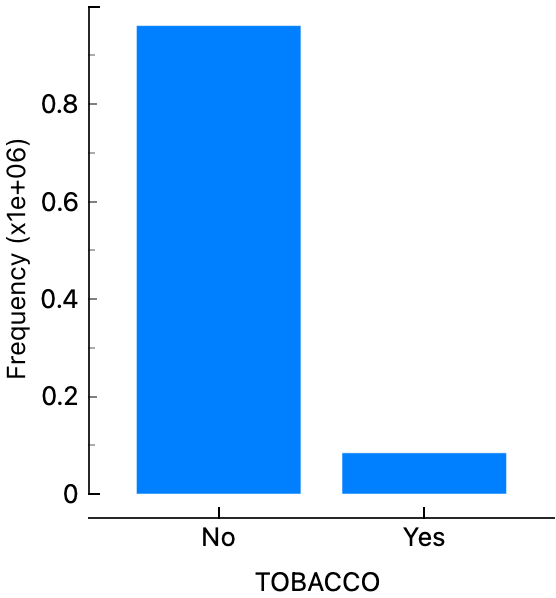
\includegraphics[width=0.44\textwidth]{img/appendix/feature_tobacco.png} 
\\ \hline
\textbf{intubed} & \\
Whether the patient was connected to the ventilator. Values:
\begin{description}
    \item[1] Yes;
    \item[2] No;
    \item[97] Missing value;
    \item[99] Missing value.
\end{description}
We have 82\% cases with missing data (Probably patients that were not hospitalized or not followed by clinics).
And we have 17\% of population was intubed (Around 40000 in one million. The 17\% is measured based on the populated data (18\% of the population)).
& 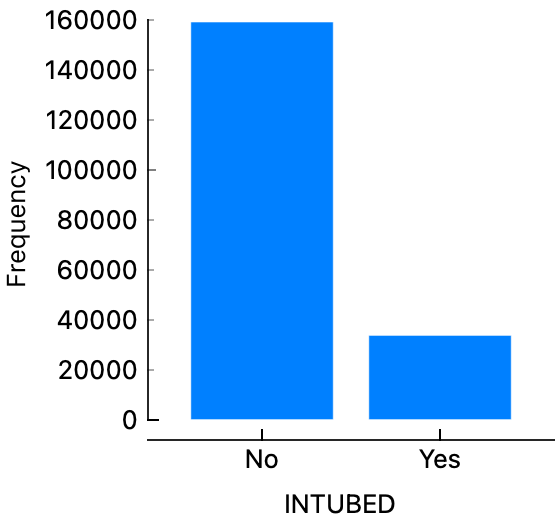
\includegraphics[width=0.44\textwidth]{img/appendix/feature_intubed.png} 
\\ \hline
\textbf{icu} & \\
Indicates whether the patient had been admitted to an Intensive Care Unit. Values:
\begin{description}
    \item[1] Yes;
    \item[2] No;
    \item[97] Missing value;
    \item[99] Missing value.
\end{description}
We have 82\% cases with missing data (Probably patients that were not hospitalized or not followed by clinics).
And we have 8\% of population was in ICU (Around 17000 in one million. The 17\% is measured based on the populated data (18\% of the population)).
& 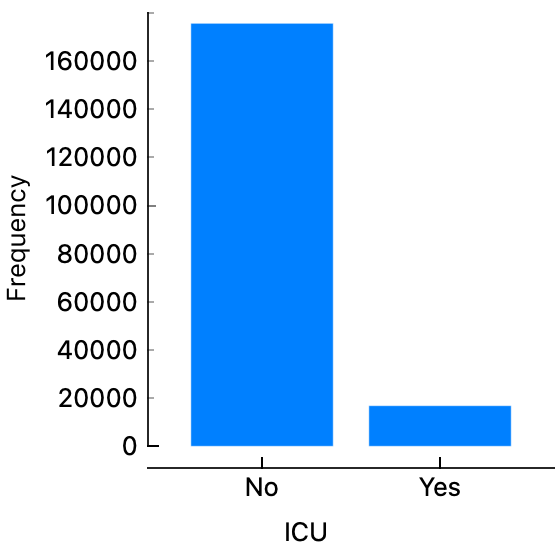
\includegraphics[width=0.44\textwidth]{img/appendix/feature_icu.png} 
\\ \hline
\textbf{date died} & \\
If the patient died indicate the date of death, and 9999-99-99 otherwise.
And we have 8\% death.
& 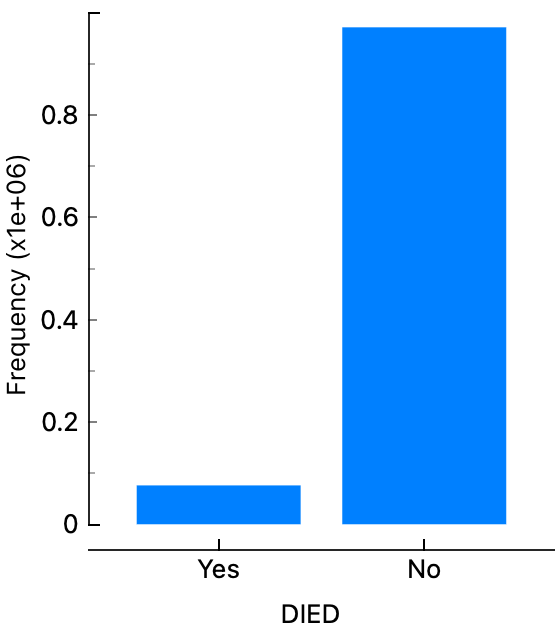
\includegraphics[width=0.44\textwidth]{img/appendix/feature_died.png} 
\\ \hline
\end{longtable}

\subsection{Feature Statistics}

\begin{figure}[H]
\caption{COVID-19 Feature Statistics}
\label{fig:feature_summary}
\centering
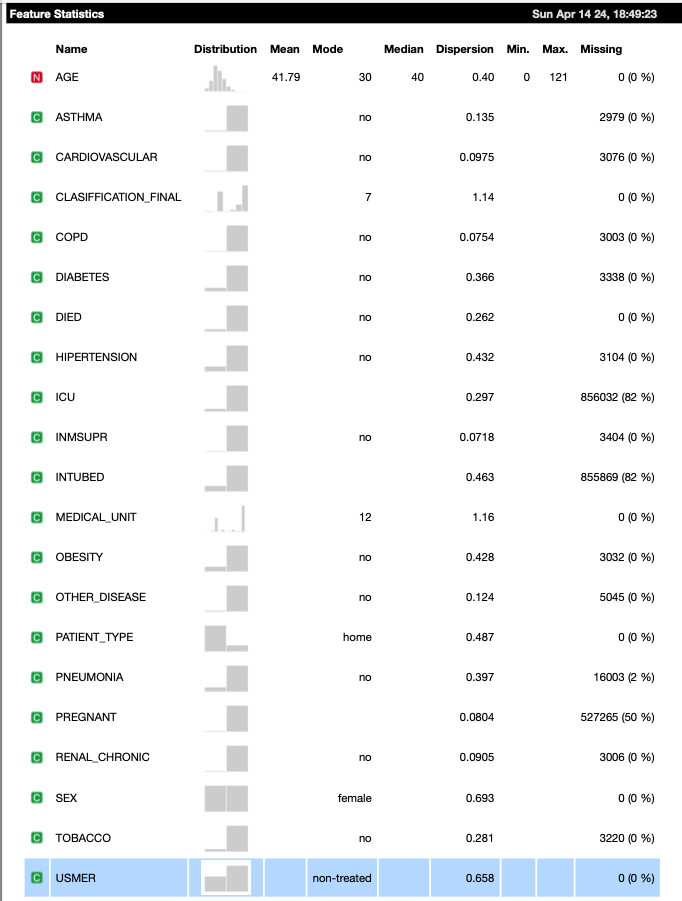
\includegraphics[width=\textwidth]{img/appendix/feature_summary.png}
\end{figure}

\newpage
\subsection{Feature Insights}

\begin{figure}[H]%
    \caption{Age by Disease (Probability Histograms)}%
    \label{fig:age_insights}%
    \centering
    \subfloat[\centering Renal]{{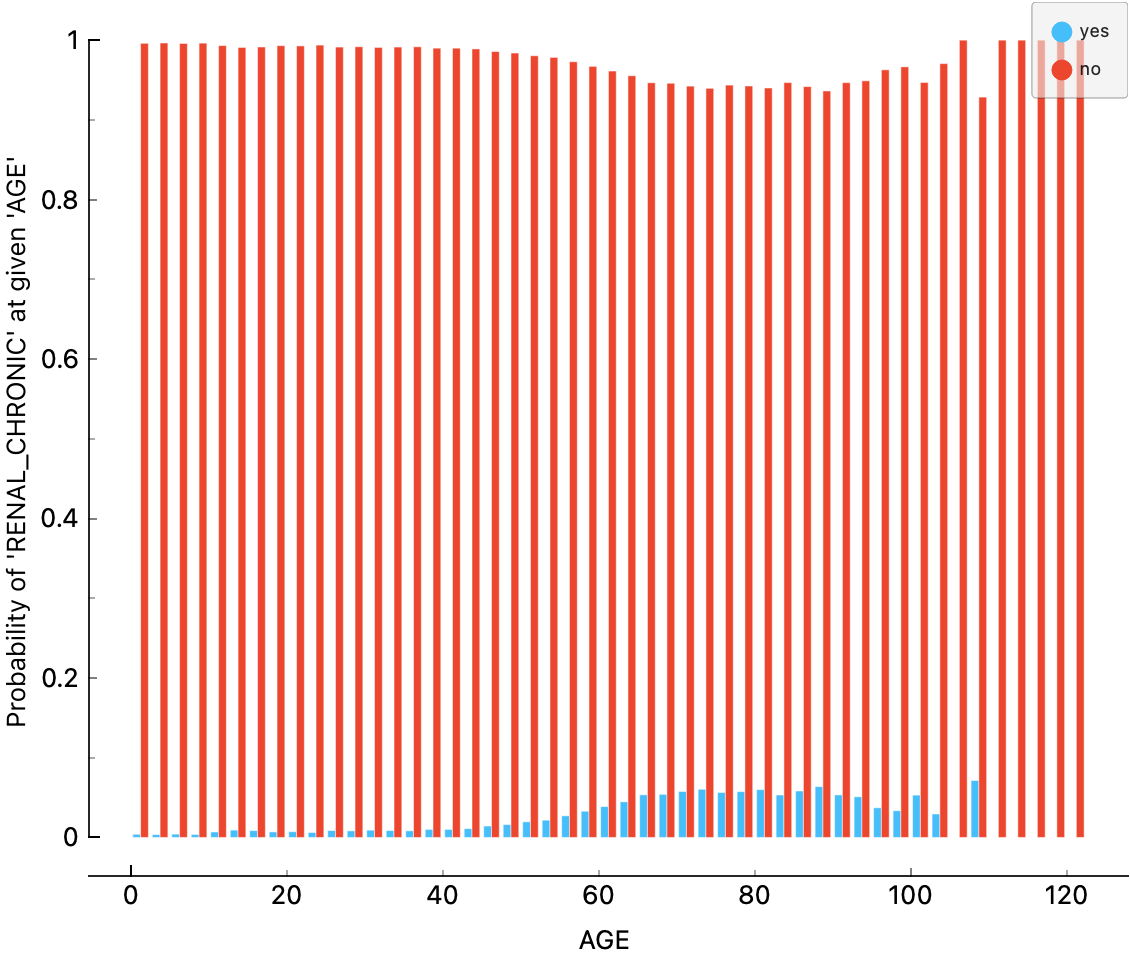
\includegraphics[width=0.45\textwidth]{img/appendix/insight_age_renal.png} }}%
    \qquad
    \subfloat[\centering Cardio]{{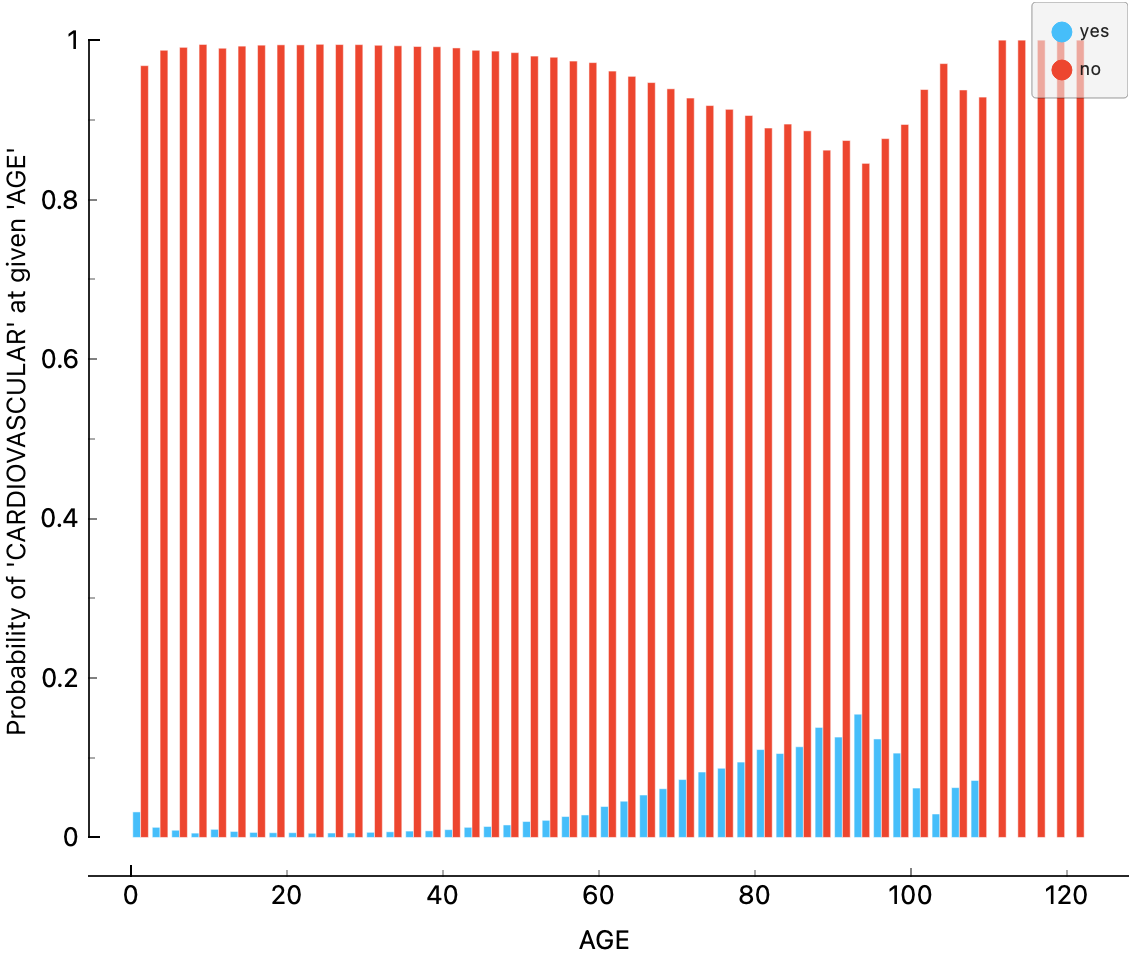
\includegraphics[width=0.45\textwidth]{img/appendix/insight_age_cardio.png} }}%
    \qquad
    \subfloat[\centering Hypertension]{{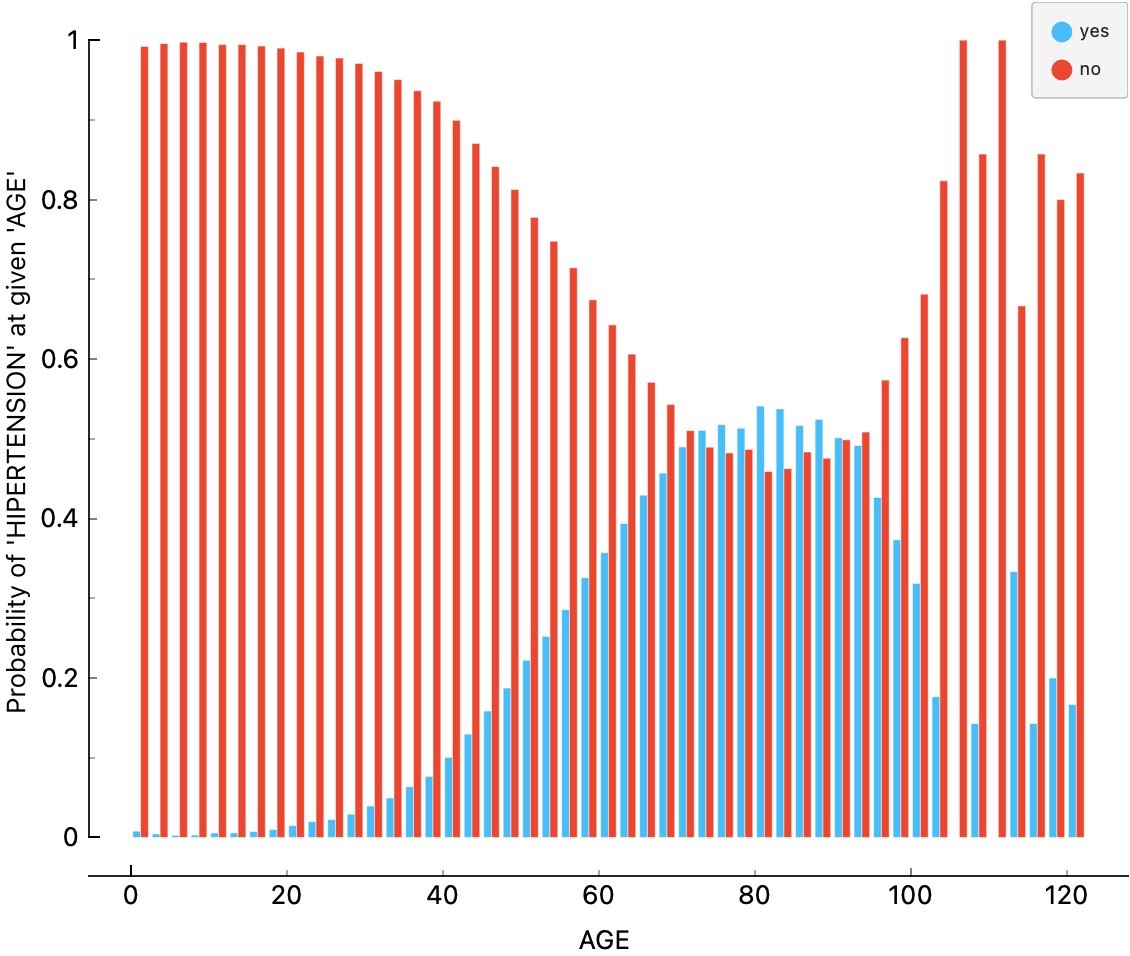
\includegraphics[width=0.45\textwidth]{img/appendix/insight_age_hipertension.png} }}% 
    \qquad
    \subfloat[\centering COPD]{{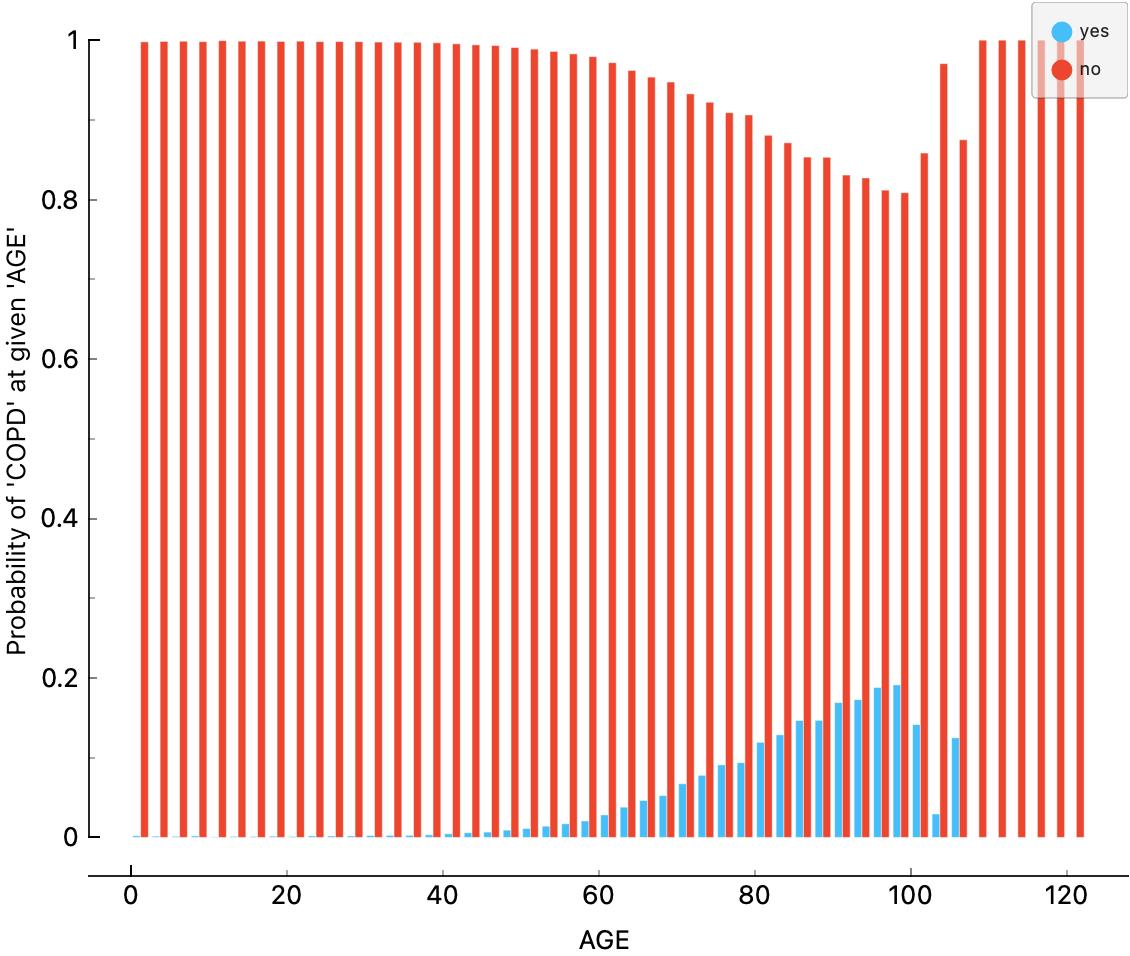
\includegraphics[width=0.45\textwidth]{img/appendix/insight_age_copd.png} }}%
    \qquad
    \subfloat[\centering Diabetes]{{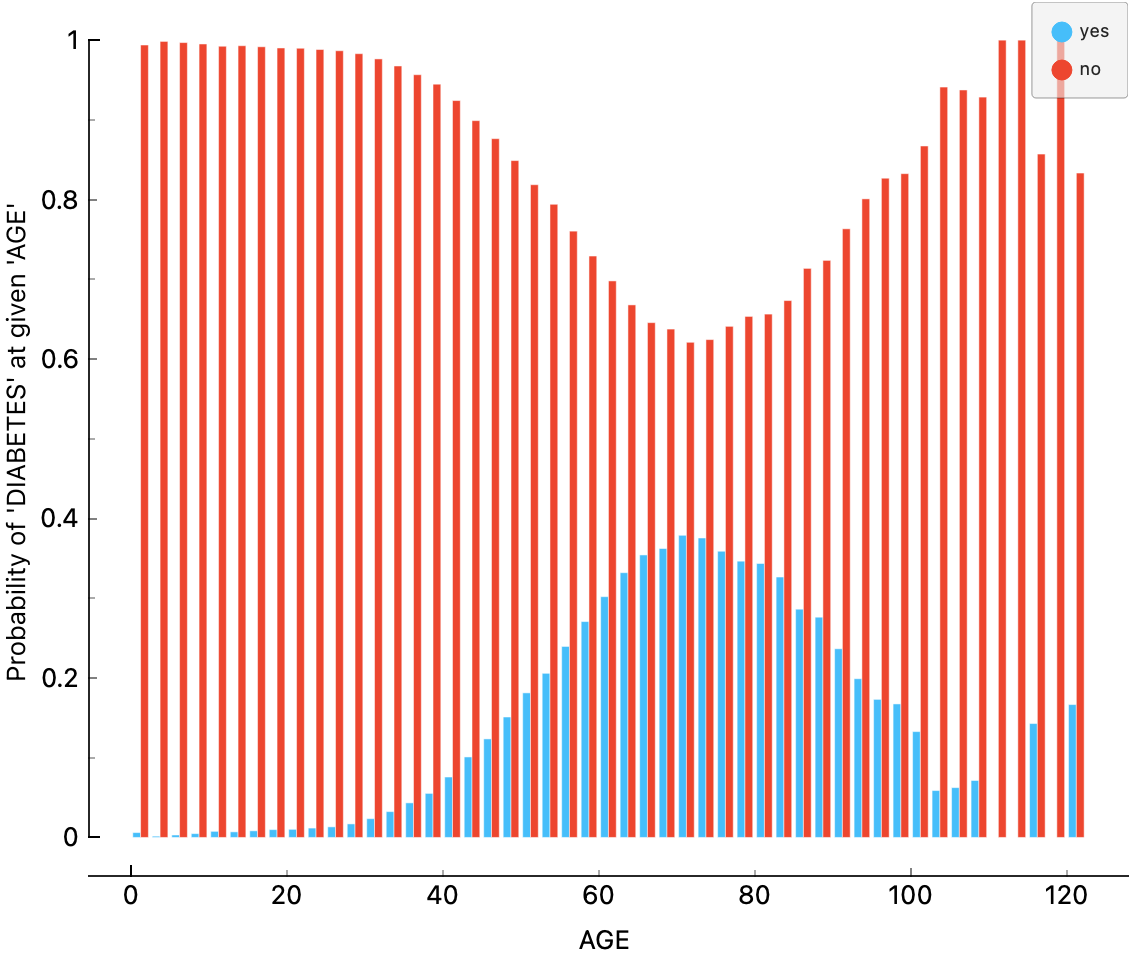
\includegraphics[width=0.45\textwidth]{img/appendix/insight_age_diabetes.png} }}%
    \qquad
    \subfloat[\centering Pneumonia]{{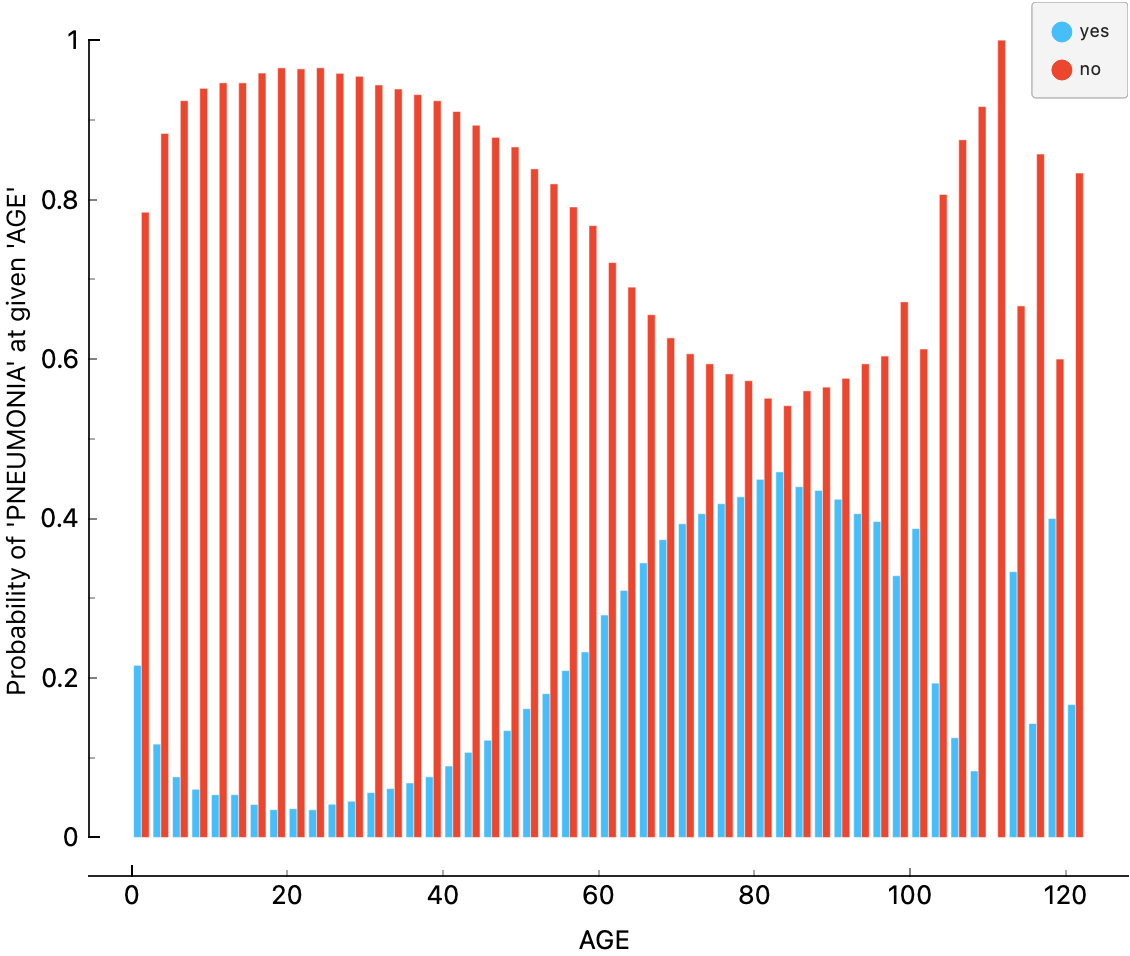
\includegraphics[width=0.45\textwidth]{img/appendix/insight_age_pneumonia.png} }}%
\end{figure}

\subsection{Feature Correlation Matrix}
\begin{figure}[H]%
    \caption{Feature Correlation Matrix}%
    \label{fig:feat_corr_matrix}%
    \centering
    {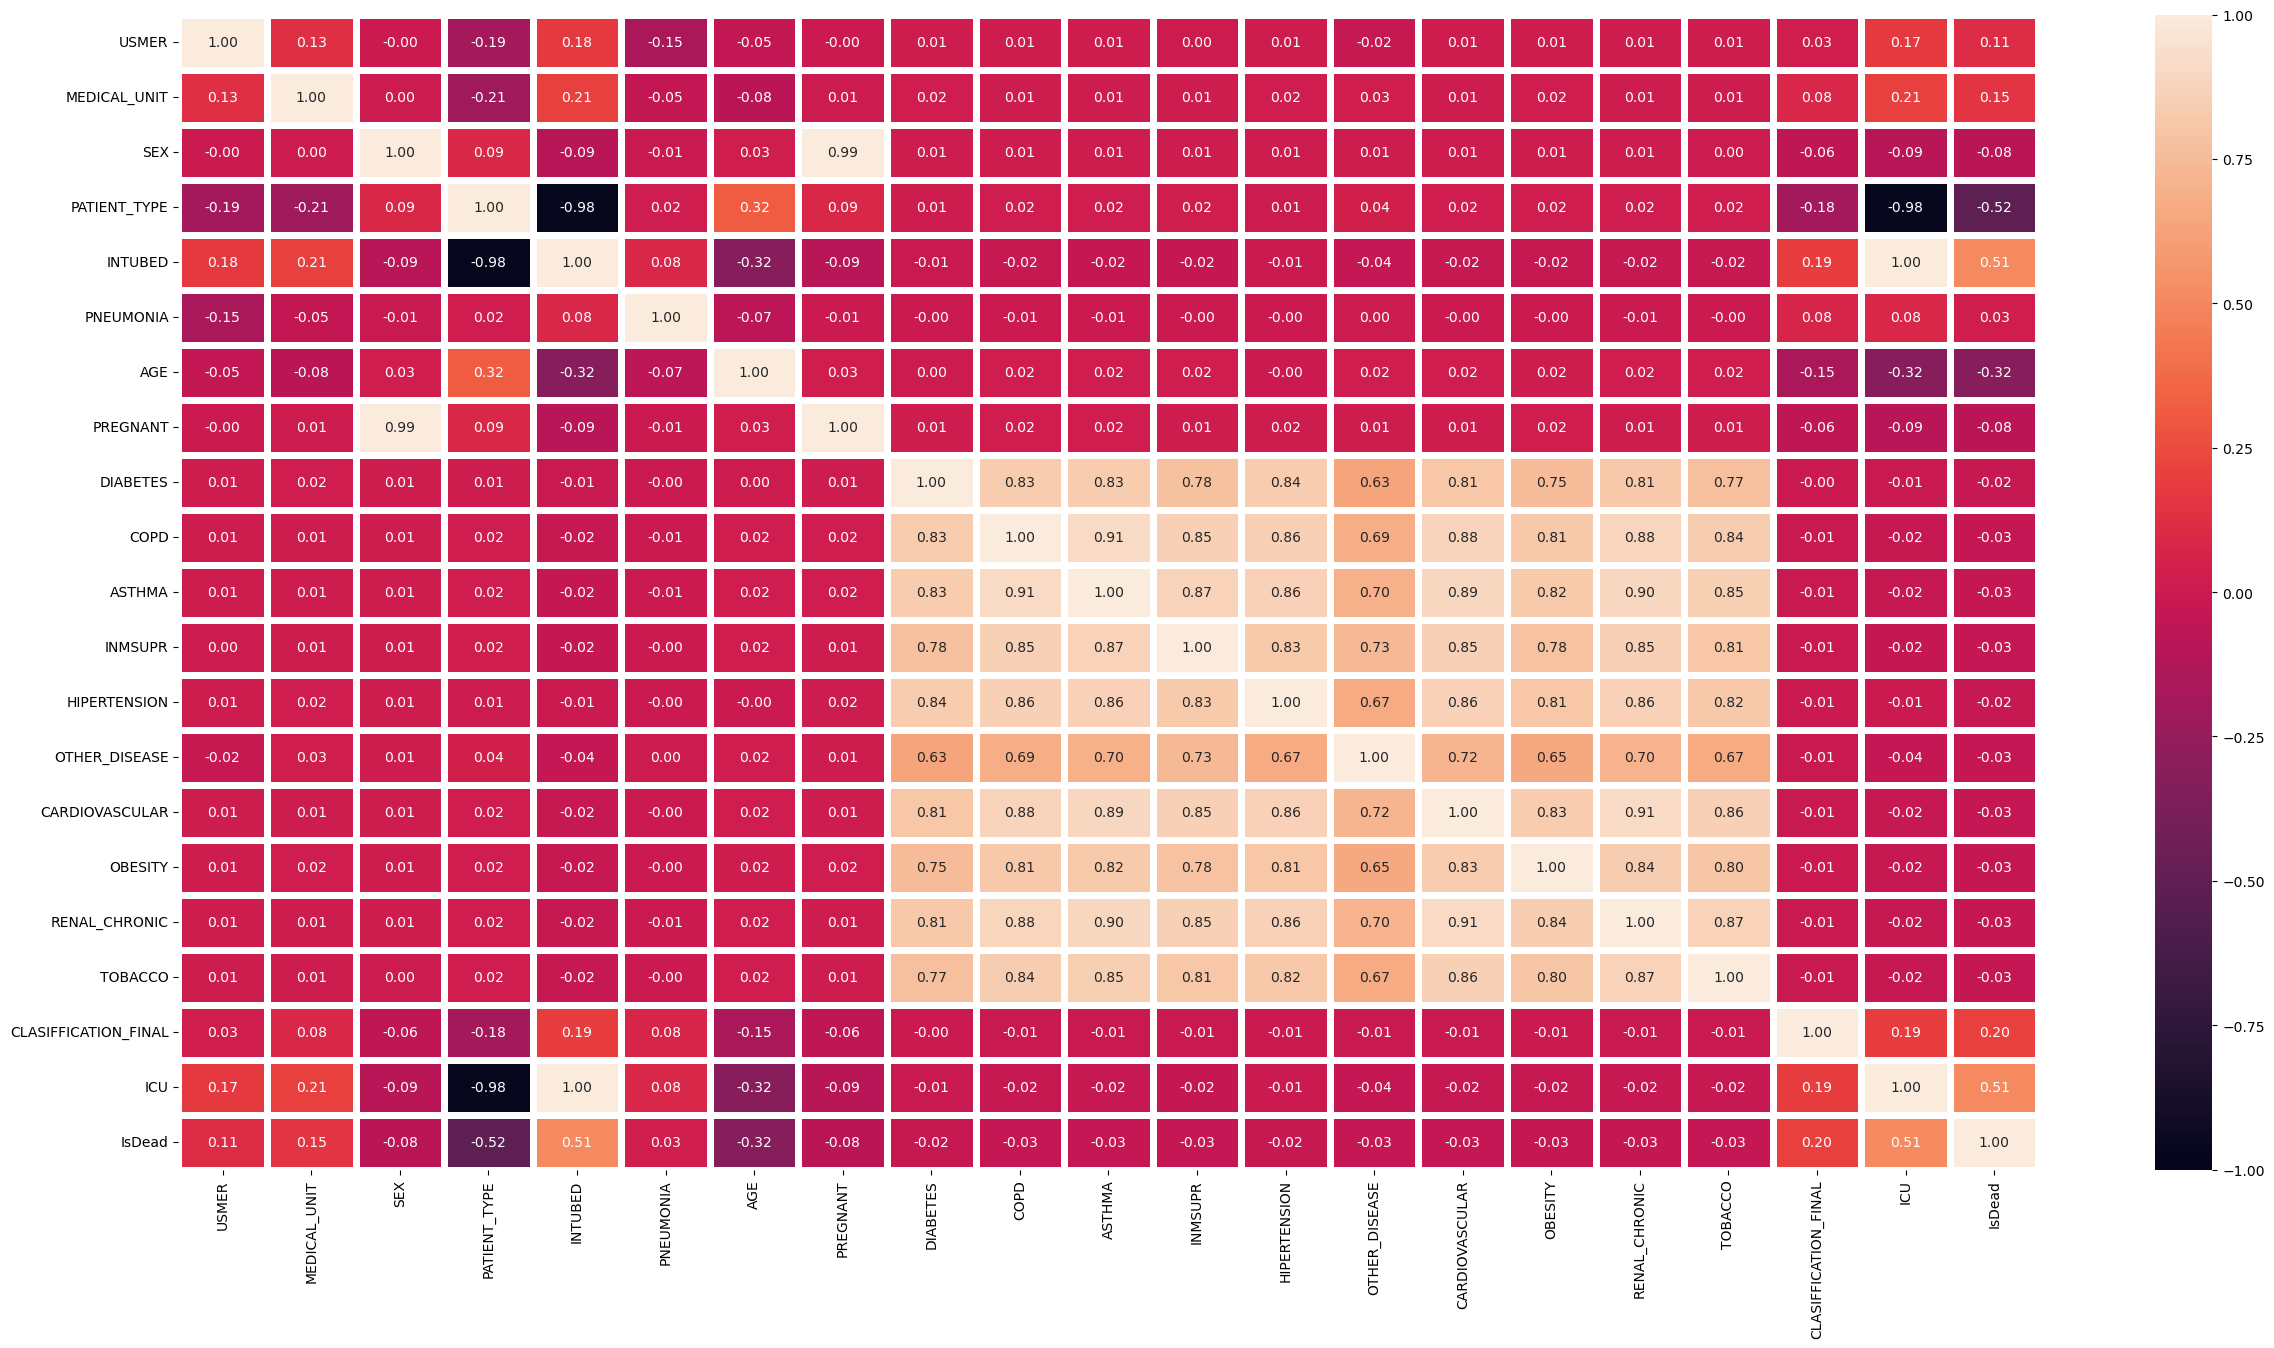
\includegraphics[angle=90, height=21cm]{img/appendix/insights_correlation_matrix.png} }
\end{figure}

\newpage
\subsection{Feature Ranking}
\begin{figure}[H]%
    \caption{Feature Ranking}%
    \label{fig:feat_full_rank}%
    \centering
    {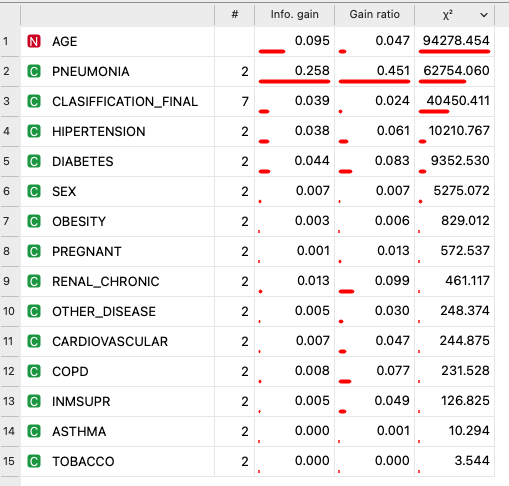
\includegraphics[width=\textwidth]{img/appendix/feat_rank.png} }
\end{figure}

\subsection{Feature Importance per Metric}

\subsubsection{AUC}
\begin{figure}[H]%
    \caption{Feature Importance for AUC}%
    \label{fig:fi_auc_10}%
    \centering
    \subfloat[\centering Catboost]{{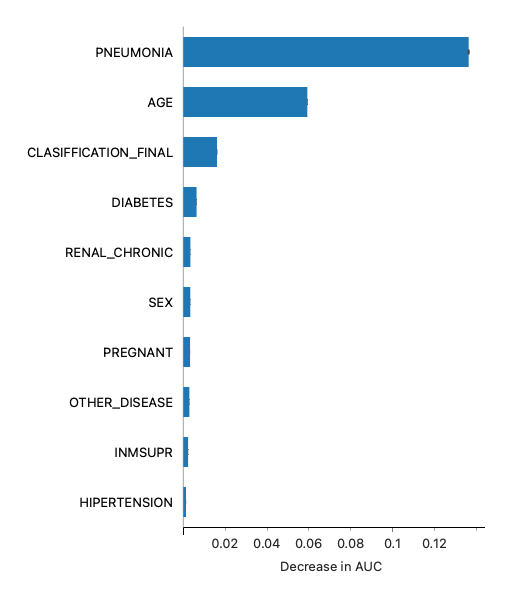
\includegraphics[width=0.45\textwidth]{img/appendix/FI_GB_AUC_10.png} }}%
    \qquad
    \subfloat[\centering Neural Network]{{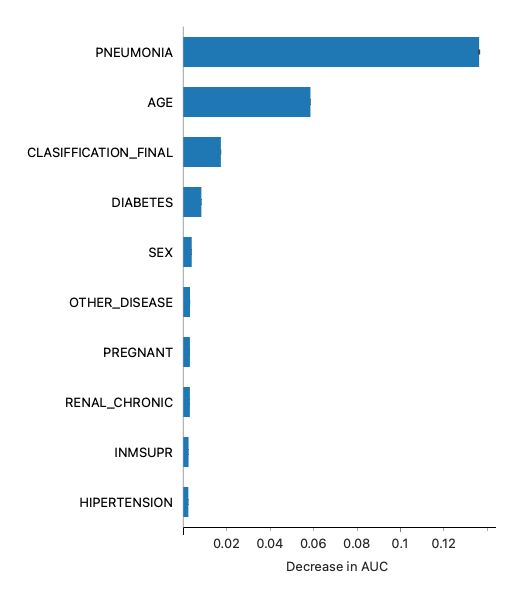
\includegraphics[width=0.45\textwidth]{img/appendix/FI_NN_AUC_10.png} }}%
    \qquad
    \subfloat[\centering Random Forest]{{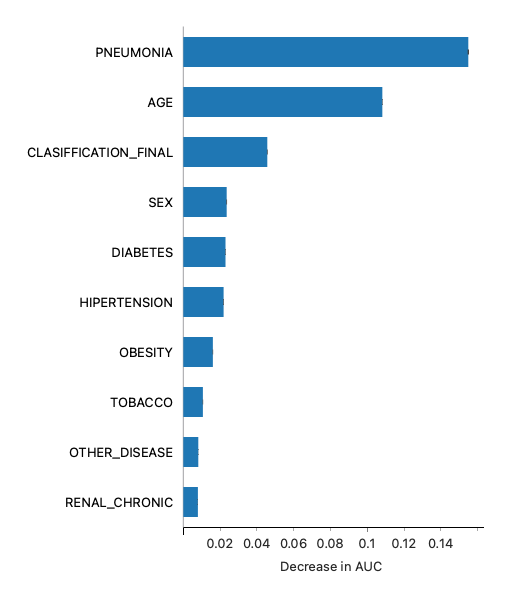
\includegraphics[width=0.45\textwidth]{img/appendix/FI_RF_AUC_10.png} }}% 
\end{figure}

\subsubsection{Precision}
\begin{figure}[H]%
    \caption{Feature Importance for Precision}%
    \label{fig:fi_prec_10}%
    \centering
    \subfloat[\centering Catboost]{{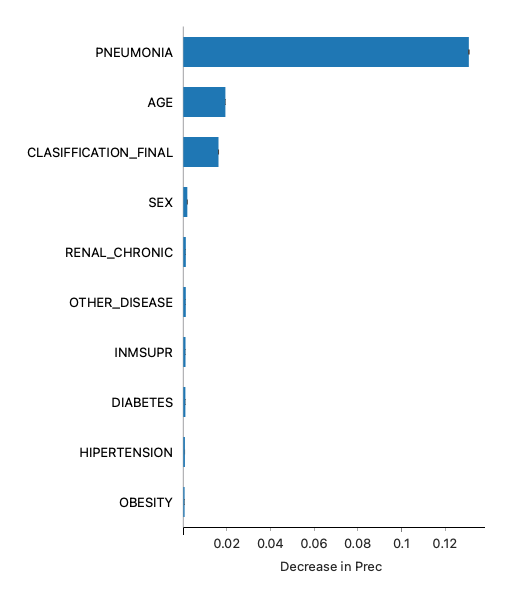
\includegraphics[width=0.45\textwidth]{img/appendix/FI_GB_Prec_10.png} }}%
    \qquad
    \subfloat[\centering Neural Network]{{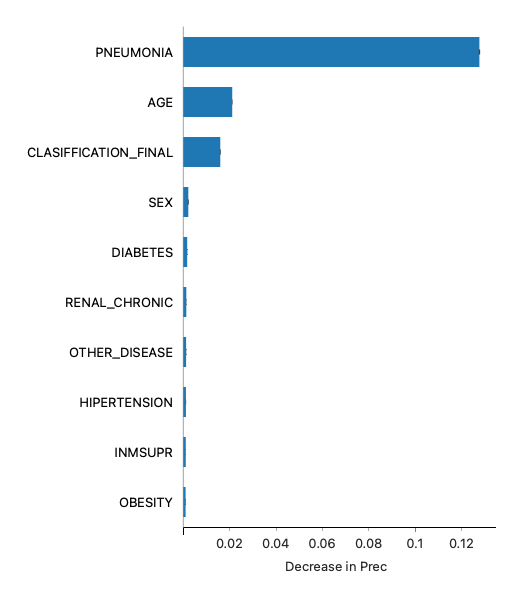
\includegraphics[width=0.45\textwidth]{img/appendix/FI_NN_Prec_10.png} }}%
    \qquad
    \subfloat[\centering Random Forest]{{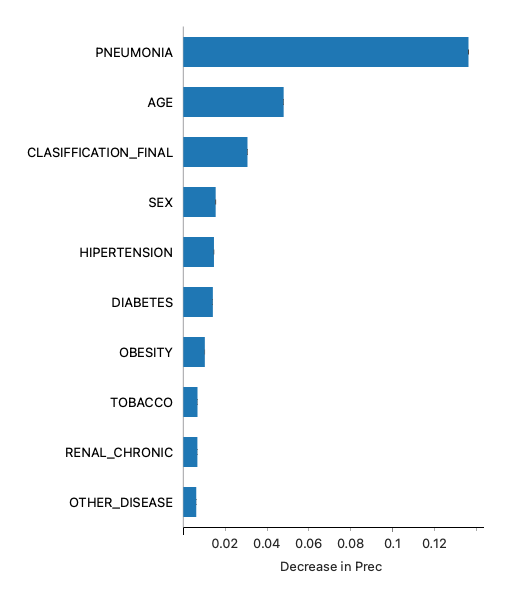
\includegraphics[width=0.45\textwidth]{img/appendix/FI_RF_Prec_10.png} }}% 
\end{figure}

\subsubsection{Recall}
\begin{figure}[H]%
    \caption{Feature Importance for Recall}%
    \label{fig:fi_recall_10}%
    \centering
    \subfloat[\centering Catboost]{{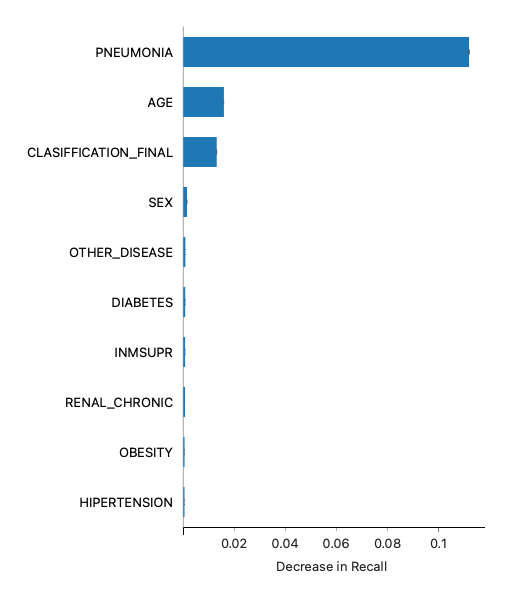
\includegraphics[width=0.45\textwidth]{img/appendix/FI_GB_Recall_10.png} }}%
    \qquad
    \subfloat[\centering Neural Network]{{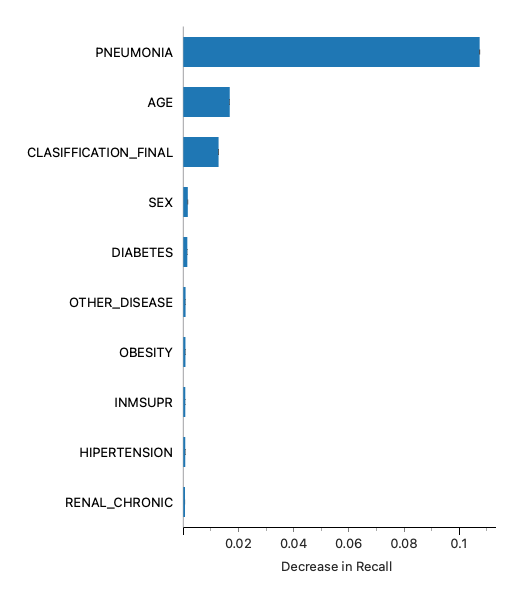
\includegraphics[width=0.45\textwidth]{img/appendix/FI_NN_Recall_10.png} }}%
    \qquad
    \subfloat[\centering Random Forest]{{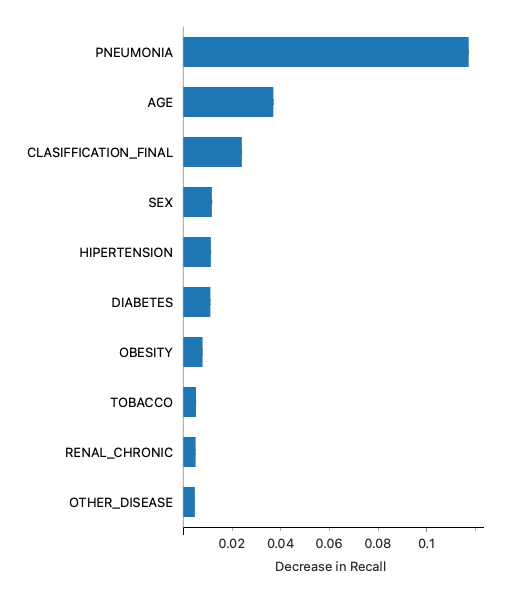
\includegraphics[width=0.45\textwidth]{img/appendix/FI_RF_Recall_10.png} }}% 
\end{figure}

\subsection{Feature Normalization Using Orange Data Mining}

\begin{figure}[H]%
    \caption{Data Preparation using Edit Domain Widget}%
    \label{fig:data_preparation_edit_dm}%
    \centering
    {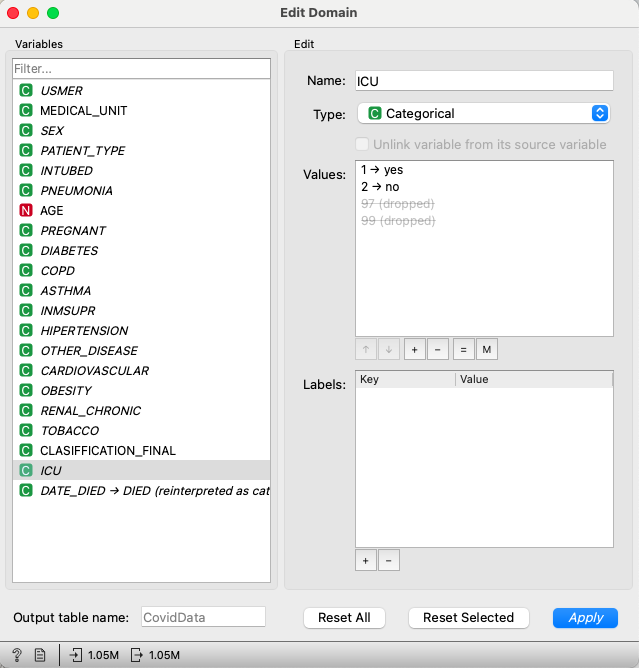
\includegraphics[width=\textwidth]{img/appendix/data_preparation_edit_domain.png} }
\end{figure}

\begin{figure}[H]%
    \caption{Data Preparation using Using Formula Widget}%
    \label{fig:data_preparation_using_formula}%
    \centering
    {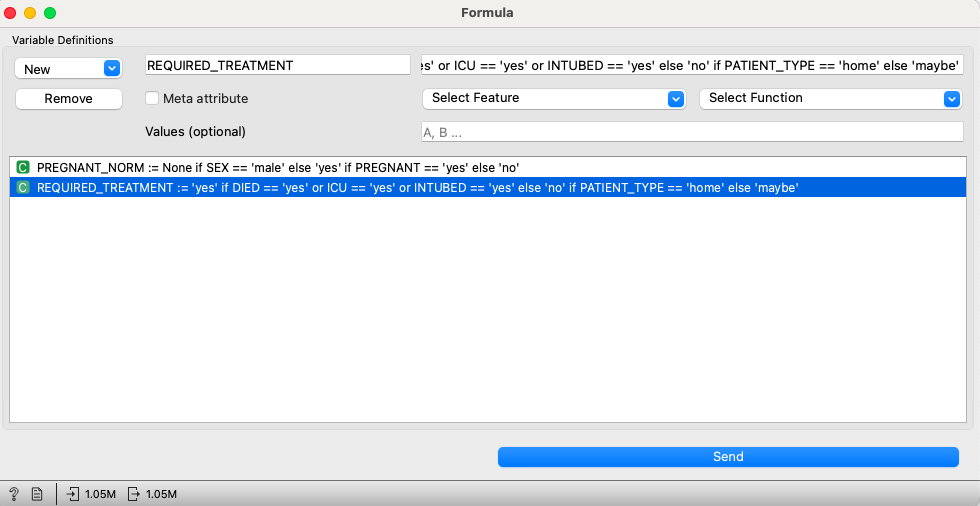
\includegraphics[width=\textwidth]{img/appendix/data_preparation_using_formula.png} }
\end{figure}

\subsection{Code Listings}

\subsection{Feature Analysis Correlation Matrix}

\begin{listing}[H]
\caption{Correlation Matrix For Feature Analysis}
\label{lst:corr_matrix}
\begin{minted}[linenos]{python}
import pandas as pd
import matplotlib.pyplot as plt
import seaborn as sns
data = pd.read_csv("CovidData.csv")
data.describe().T
data['IsDead'] = data['DATE_DIED'].apply(lambda x: 1 if x == '9999-99-99' else 0)
data = data.drop(["DATE_DIED"], axis = 1)

plt.figure(figsize=(30, 15))
sns.heatmap(data.corr(), vmin=-1, vmax=1, cbar = True,
            linewidths = 5, 
            annot = True,
            fmt=".2f")
plt.show()
\end{minted}
\end{listing}

\subsubsection{Feature Normalization}

\begin{listing}[H]
\caption{Feature Normalization For COVID-19 Dataset - Functions}
\label{lst:feat_norm_functions}
\begin{minted}[linenos]{scala}
def makeBool(value: String): String = value match {
    case "1" => "yes"
    case "2" => "no"
    case _ => ""
}

def makeDate(value: String): String = value match {
    case "9999-99-99" => ""
    case _ => value
}

def makeSex(value: String): String = value match {
    case "1" => "female"
    case "2" => "male"
}

def makeDied(value: String): String = value match {
    case "9999-99-99" => "no"
    case _ => "yes"
}

def makeRequiredTreatment(dateDied: String, icu: String, 
                          intubed: String, patientType: String)
                          : String = {
    if (dateDied != "9999-99-99") "yes"
    else if (icu == "1") "yes"
    else if (intubed == "1") "yes"
    else if (patientType == "1") "no"
    else "maybe"
}

def makePatientType(patientType: String): String = patientType match {
    case "1" => "home"
    case "2" => "hospital"
}
\end{minted}
\end{listing}

\begin{listing}[H]
\caption{Feature Normalization For COVID-19 Dataset - Process}
\label{lst:feat_norm_process}
\begin{minted}[linenos]{scala}
    Array(usmer, 
          medicalUnit, 
          makeSex(sex), 
          makePatientType(patientType), 
          makeDate(dateDied), 
          makeBool(intubed), 
          makeBool(pneumonia), 
          age, 
          if (makeSex(sex) == "male") "na" else makeBool(pregnant), 
          makeBool(diabetes), 
          makeBool(copd), 
          makeBool(asthma), 
          makeBool(inmsupr), 
          makeBool(hipertension), 
          makeBool(other_disease), 
          makeBool(cardiovascular), 
          makeBool(obesity), 
          makeBool(renal_chronic), 
          makeBool(tobacco), 
          clasiffication_final, 
          makeBool(icu),
          makeDied(dateDied),
          makeRequiredTreatment(dateDied, icu, intubed, patientType)).mkString(",")
}
\end{minted}
\end{listing}


